\documentclass[10pt]{beamer}
\usepackage{kotex}
\usepackage{commath}
\usepackage{multirow}
\usepackage{multicol}
\usepackage{arydshln} % Include this package
\usepackage{bbding}

\usepackage{tikz}
\usepackage{tikz-cd}
\usetikzlibrary{math} % for calculations
\usetikzlibrary{shapes, arrows.meta, positioning, shadows}
\usetikzlibrary{arrows,shapes.geometric}  % Optional, based on your needs
\usetikzlibrary{3d, calc}
\usetikzlibrary{matrix, positioning, arrows.meta, shapes.multipart, chains}
\usetikzlibrary{decorations.pathreplacing,calligraphy}
\usetheme[progressbar=frametitle]{metropolis}
\usepackage{appendixnumberbeamer}

\usepackage{adjustbox}
\usepackage{booktabs}
\usepackage[scale=2]{ccicons}

\usepackage{tcolorbox}

\usepackage{pgfplots}
\usepgfplotslibrary{fillbetween}
\pgfplotsset{compat=1.15}
\usepgfplotslibrary{dateplot}

\usepackage{xspace}
\newcommand{\themename}{\textbf{\textsc{metropolis}}\xspace}

\usepackage[linesnumbered,ruled]{algorithm2e}
\usepackage{algpseudocode}
\usepackage{setspace}
\SetKwComment{Comment}{/* }{ */}
\SetKwProg{Fn}{Function}{:}{end}
\SetKw{End}{end}
\SetKw{DownTo}{downto}

% Define a new environment for algorithms without line numbers
\newenvironment{algorithm2}[1][]{
	% Save the current state of the algorithm counter
	\newcounter{tempCounter}
	\setcounter{tempCounter}{\value{algocf}}
	% Redefine the algorithm numbering (remove prefix)
	\renewcommand{\thealgocf}{}
	\begin{algorithm}
	}{
	\end{algorithm}
	% Restore the algorithm counter state
	\setcounter{algocf}{\value{tempCounter}}
}

\usepackage{xcolor}   % Required for specifying colors

\usepackage{listings} %Code
\renewcommand{\lstlistingname}{Code}%
\definecolor{keyword}{RGB}{255, 0, 0}
\definecolor{identifier}{RGB}{0, 0, 255}
\definecolor{comment}{RGB}{0, 128, 0}
\definecolor{string}{RGB}{163, 21, 21}

\lstdefinestyle{c}{
	language=C,
	basicstyle=\ttfamily\small,
	keywordstyle=\color{keyword},
	identifierstyle=\color{identifier},
	commentstyle=\color{comment}\itshape,
	stringstyle=\color{string},
	showstringspaces=false,
	%	numberstyle=\tiny\color{gray},
	%	numbersep=5pt,
	frame=single,
	tabsize=4,
	captionpos=b,
	breaklines=true,
	breakatwhitespace=true,
	%	numbers=left
}

\usepackage{amsthm, amsmath}


\newcommand{\cyclic}[1]{\langle #1 \rangle}
\newcommand{\uniform}{\overset{\$}{\leftarrow}}
\newcommand{\N}{\mathbb{N}}
\newcommand{\Z}{\mathbb{Z}}
\newcommand{\Q}{\mathbb{Q}}
\newcommand{\R}{\mathbb{R}}
\newcommand{\C}{\mathbb{C}}
\newcommand{\F}{\mathbb{F}}

\newcommand{\xmark}{\textcolor{red}{\XSolidBrush}}
\newcommand{\vmark}{\textcolor{green!75!black}{\CheckmarkBold}}

\title{\huge\bf Software Verification}
\subtitle{\textcolor{magenta}{\textbf{Lecture 01. Introduction to Software Analysis}}}
% \date{\today}
\date{}
\author{\large\textcolor{cyan}{\bf Ji, Yong-Hyeon}\\ \\ \small 24. 07. 11 (Thu)}
\institute{\small
	Coding \& Optimization Together (CO2) \\
	Crypto \& Security Engineering Lab (CSE) \\
	Department of Information Security, Cryptology, and Mathematics
}
% \titlegraphic{\hfill\includegraphics[height=1.5cm]{logo.pdf}}

\begin{document}
	
	\maketitle
	
	\begin{frame}{Table of Contents}
		\setbeamertemplate{section in toc}[sections numbered]
		\tableofcontents%[hideallsubsections]
	\end{frame}
	
	\section{Motivation}
	\begin{frame}{1. Motivation}
		\begin{enumerate}
			\item Software systems are mostly \underline{\bf unsafe}.
			\item[]
			\item Software errors cost the U.S. economy \$60B ($\approx 82\text{조}$) every year. 
			\begin{itemize}
				\item[]
				\item[(1996)] Explosion of the Arian-5 rocket. \$8 billion ($\approx 11\text{조}$)
				\item[]
				\item[(1998)] NASA’s Mars climate orbiter lost in space. \$125 million ($\approx 1700\text{억}$)
				\item[]
				\item[(2000)] Accidents in radiation therapy system. 8 patients died 
				\item[]
				\item[(2007)] Air control system shutdown in LA airport. 6,000 passengers stranded 
				\item[]
				\item[(2012)] Glitch in trading software of Knight Captal. \$440 million ($\approx 6000\text{억}$)
				\item[]
				\item[(2014)] Airbag malfunction of Nissan vehicles. \$1 million vehicles recalled
			\end{itemize}
		\end{enumerate}
	\end{frame}
	\begin{frame}{1. Motivation}
		\begin{enumerate}
			\item[3.] Current Technologies for Safe Software
			\begin{enumerate}[(a)]
				\item[]
				\item Code Review
				\item[]
				\item Testing
				\item[]
				\item Debugging
				\item[]
				\item Simulation
				\item[]
				\item $\cdots$
			\end{enumerate}
		\end{enumerate}
	\end{frame}

	\section{Software Analysis}
	\subsection{2.1 Software Analysis}
	\begin{frame}{2.1 Software Analysis}
		\begin{itemize}
			\item Technology for catching bugs or proving correctness of software. \\ \vspace{24pt}
			\begin{center}\adjustbox{scale=1}{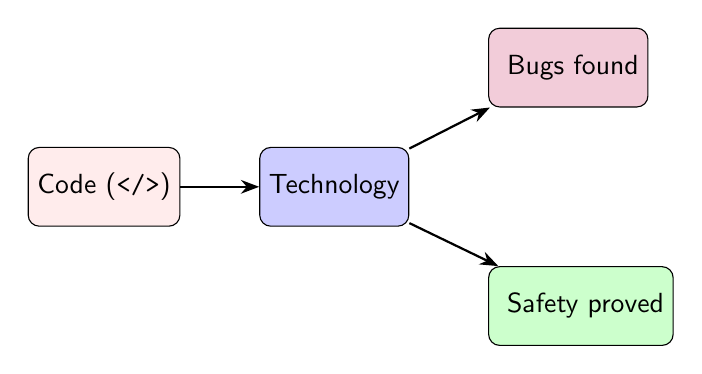
\begin{tikzpicture}[
				node distance=.5cm and 1cm,
				process/.style={rectangle, rounded corners, draw, minimum width=1.5cm, minimum height=1cm, text centered, font=\sffamily},
				arrow/.style={-Stealth, thick},
				pastelgreen/.style={fill=green!20},
				pastelblue/.style={fill=blue!20},
				pastelpink/.style={fill=pink!30},
				pastelpurple/.style={fill=purple!20}
				]
				
				% Nodes
				\node (F) [process, pastelpink] {Code (\texttt{</>})};
				\node (SATsolver) [process, pastelblue, right=of F] {Technology};
				\node (SAT) [process, pastelgreen, below right=of SATsolver] {\textcolor{green!50!black}{\CheckmarkBold}\ Safety proved};
				\node (UNSAT) [process, pastelpurple, above right=of SATsolver] {\textcolor{red}{\XSolidBrush}\ Bugs found};
				
				% Arrows
				\draw[arrow] (F) -- (SATsolver);
				\draw[arrow] (SATsolver) -- node[left] {} (SAT);
				\draw[arrow] (SATsolver) -- node[left] {} (UNSAT);
			\end{tikzpicture}}
			\end{center}
		\end{itemize}
	\end{frame}
	
	\subsection{2.2 A Hard Limit}
	\begin{frame}{2.2 A Hard Limit}
		\begin{itemize}
			\item The Halting problem is not computable. (Alan Turing, 1936) \vspace{24pt}
			\begin{center}\adjustbox{scale=1}{\begin{tikzpicture}[
				node distance=.25cm and 1.5cm,
				process/.style={rectangle, rounded corners, draw, minimum width=1.5cm, minimum height=1cm, text centered, font=\sffamily},arrow/.style={-Stealth, thick},
				]
				
				% Nodes
				\node (A) [] {program};
				\node (B) [right=of F] {Halting Algorithm};
				\node (C) [below right=of B] {$\infty$};
				\node (D) [above right=of B] {Halt};
				
				% Arrows
				\draw[arrow] (A) -- (B);
				\draw[arrow] (B) -- node[left] {} (C);
				\draw[arrow] (B) -- node[left] {} (D);
				\end{tikzpicture}}
			\end{center}
		\end{itemize}
	\end{frame}
	\begin{frame}{2.2 A Hard Limit}
		\begin{itemize}
			\item If exact analysis is possible, we can solve the Halting problem.
			\begin{center}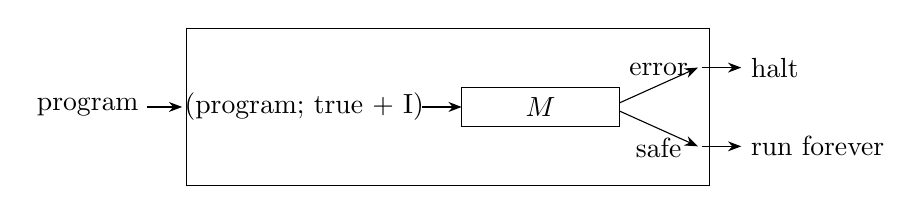
\begin{tikzpicture}
					\draw[black] (-1,-.25) rectangle (1,.25);
					\node at (0,0) {$M$};
					\draw[arrows=-Stealth] (1,.05) -- (2,.5) node[midway, above] {error};
					\draw[arrows=-Stealth] (1,-.05) -- (2,-.5) node[midway, below] {safe};
					\draw[arrows=-Stealth] (2.05,.5) -- (2.55,.5) node[right] {halt};
					\draw[arrows=-Stealth] (2.05,-.5) -- (2.55,-.5) node[right] {run forever};
					\draw[arrows=-Stealth] (-1.5,0) -- (-1,0);
					\node at (-3,0) {(program; true + I)};
					\draw[arrows=-Stealth] (-5,0) -- (-4.55,0);
					\node at (-5.75,0) {program};
					\draw[black] (-4.5,-1) rectangle (2.15,1);
			\end{tikzpicture}\end{center}
			\item[]
			\item Rice's Theorem (1951): any non-trivial semantic property of a program is undecidable.
		\end{itemize}
	\end{frame}

	\subsection{2.3 Trade-off}
	\begin{frame}{2.3 Trade-off}
		\begin{itemize}
			\item Three desirable properties
			\begin{itemize}
				\item \textcolor{red}{\bf Soundness}: all program behaviors are captured
				\item \textcolor{blue}{\bf Completeness}: only program behaviors are captured
				\item \textcolor{green!75!black}{\bf Automation}: without human intervention
			\end{itemize}
			\item[]
			\item Achieving all of them is generally infeasible \\
			\begin{center}\adjustbox{scale=.75}{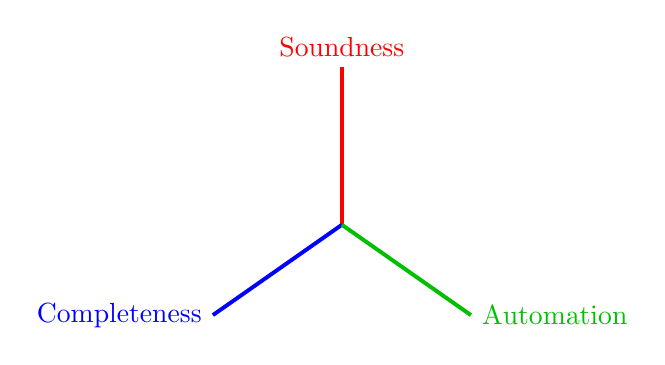
\begin{tikzpicture}
					\draw[red, line width=.5mm] (0,0) -- (0,2) node[above] {Soundness};
					\draw[blue, line width=.5mm,rotate=125] (0,0) -- (0,2) node[above, left] {Completeness};
					\draw[green!75!black, line width=.5mm, rotate=-125] (0,0) -- (0,2) node[above, right] {Automation};
			\end{tikzpicture}}\end{center}
		\end{itemize}
	\end{frame}
	\begin{frame}{2.3 Trade-off}
		\begin{itemize}
			\item Completeness + Automation (Testing)
			\ \begin{center}\adjustbox{scale=.75}{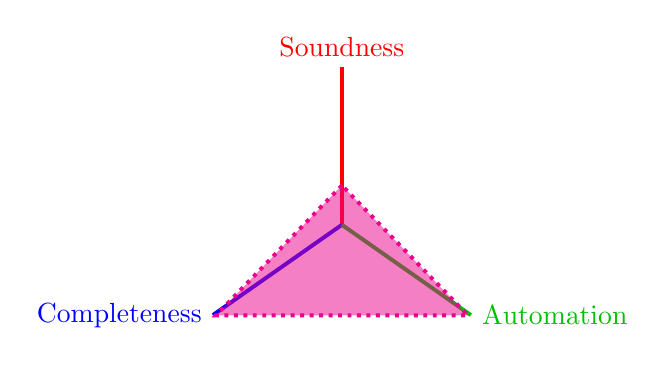
\begin{tikzpicture}
				\draw[red, line width=.5mm] (0,0) -- (0,2) node[above] {Soundness};
				\draw[blue, line width=.5mm,rotate=125] (0,0) -- (0,2) node[above, left] {Completeness};
				\draw[green!75!black, line width=.5mm, rotate=-125] (0,0) -- (0,2) node[above, right] {Automation};
				\draw[dotted, line width=.5mm, magenta, fill=magenta, fill opacity=0.5] 
				(0,.5) -- (-1.6,-1.15) -- (1.6,-1.15) -- cycle;
			\end{tikzpicture}}\end{center}
			\item Sound + Automation (Static Analysis, Compiler)
		\ \begin{center}\adjustbox{scale=.75}{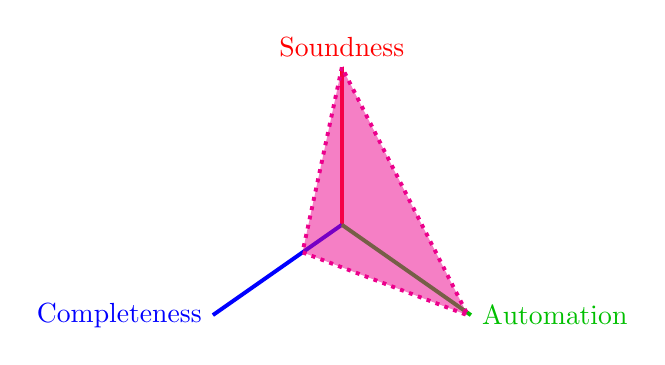
\begin{tikzpicture}
			\draw[red, line width=.5mm] (0,0) -- (0,2) node[above] {Soundness};
			\draw[blue, line width=.5mm,rotate=125] (0,0) -- (0,2) node[above, left] {Completeness};
			\draw[green!75!black, line width=.5mm, rotate=-125] (0,0) -- (0,2) node[above, right] {Automation};
			\draw[dotted, line width=.5mm, magenta, fill=magenta, fill opacity=0.5] 
			(0,2) -- (-.5,-.35) -- (1.6,-1.15) -- cycle;
	\end{tikzpicture}}\end{center}
		\end{itemize}
	\end{frame}
	\begin{frame}{2.3 Trade-off}
		\begin{itemize}
			\item Soundness + Completeness (Program Verification)
			\ \begin{center}\adjustbox{scale=.75}{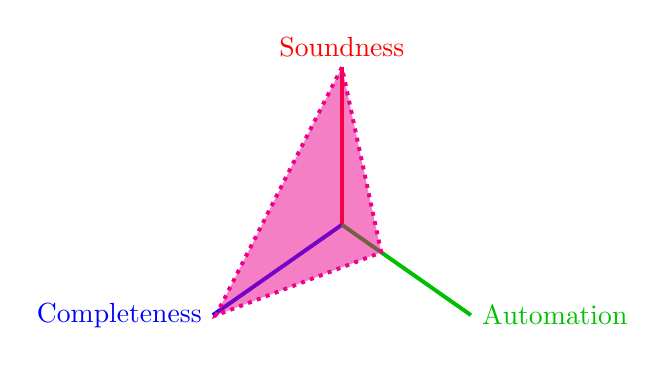
\begin{tikzpicture}
				\draw[red, line width=.5mm] (0,0) -- (0,2) node[above] {Soundness};
				\draw[blue, line width=.5mm,rotate=125] (0,0) -- (0,2) node[above, left] {Completeness};
				\draw[green!75!black, line width=.5mm, rotate=-125] (0,0) -- (0,2) node[above, right] {Automation};
				\draw[dotted, line width=.5mm, magenta, fill=magenta, fill opacity=0.5] 
				(0,2) -- (-1.6,-1.15) -- (.5,-.35) -- cycle;
			\end{tikzpicture}}\end{center}
			\item And ...
			\ \begin{center}\adjustbox{scale=.75}{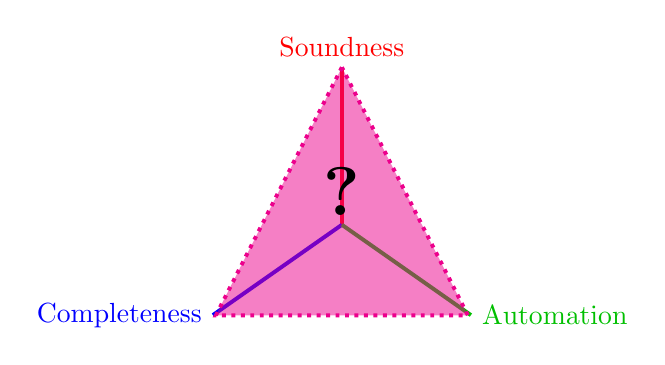
\begin{tikzpicture}
				\draw[red, line width=.5mm] (0,0) -- (0,2) node[above] {Soundness};
				\draw[blue, line width=.5mm,rotate=125] (0,0) -- (0,2) node[above, left] {Completeness};
				\draw[green!75!black, line width=.5mm, rotate=-125] (0,0) -- (0,2) node[above, right] {Automation};
				\draw[dotted, line width=.5mm, magenta, fill=magenta, fill opacity=0.5] 
				(0,2) -- (-1.6,-1.15) -- (1.6,-1.15) -- cycle;
				\node[above] (0,0) {\bf\Huge ?};
			\end{tikzpicture}}\end{center}
		\end{itemize}
	\end{frame}

	\section{Basic Principle}
	\begin{frame}{3. Basic Principle}
		\begin{itemize}
			\item Observe the program behavior by ``executing'' the program
			\begin{itemize}
				\item Report errors found during the execution
				\item When no error is found, report ``verified''
			\end{itemize}
			\item Three types of program execution:
			\begin{itemize}
				\item \textcolor{blue}{\bf Concrete execution}
				\item \textcolor{blue}{\bf Symbolic execution}
				\item \textcolor{blue}{\bf Abstract execution}
				\item and their combinations, e.g., concolic execution 
			\end{itemize}
		\end{itemize}
	\end{frame}
	\begin{frame}{3. Basic Principle}
		\begin{itemize}
			\item \textcolor{blue}{\bf Concrete} \[
			2 * 3 - 6 = 0
			\]
			\item []
			\item \textcolor{blue}{\bf Symbolic} \[
			a*b+(-c)=0
			\]
			\item []
			\item \textcolor{blue}{\bf Abstract} \[
			(\R, +, *)
			\]
		\end{itemize}
	\end{frame}

	\subsection{3.1 SW Analysis based on Concrete Execution}
	\begin{frame}{3.1 SW Analysis based on Concrete Execution}
		\textbf{Software Analysis based on Concrete Execution (Testing)}
		\begin{itemize}
			\item Execute the program with \underline{concrete inputs}, analyzing individual program states separately.
		\end{itemize}
	\end{frame}

	\begin{frame}{3.1 SW Analysis based on Concrete Execution}
		\begin{itemize}
			\item Error-triggering test? (Test Vector)
			\item[] 
			\item Probability of the error? (assume $0\leq x,y\leq 10,000$)
			\item[]
			\item \textbf{Types of Fuzzing} \begin{itemize}
				\item Blackbox Fuzzing
				\item Greybox Fuzzing
				\item Whitebox Fuzzing
			\end{itemize}
		\end{itemize}
	\end{frame}

	\subsection{3.2 SW Analysis based on Symbolic Execution}
	\begin{frame}{3.2 SW Analysis based on Symbolic Execution}
		\textbf{Software Analysis based on Symbolic Execution}
		\begin{itemize}
			\item Execute the program with \underline{symbolic inputs}, analyzing each program path only once.
		\end{itemize}
	\end{frame}
	\begin{frame}{3.2.1 Example: Symbolic Verification}
		\begin{center}\adjustbox{scale=1}{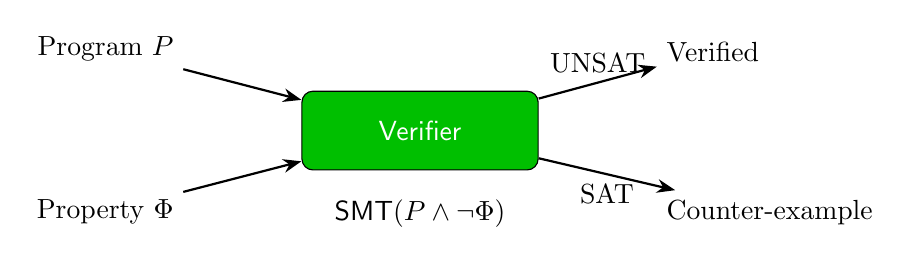
\begin{tikzpicture}[
			node distance=.25cm and 1.5cm,
			process/.style={rectangle, rounded corners, draw, minimum width=3cm, minimum height=1cm, text centered, font=\sffamily},arrow/.style={-Stealth, thick},
			]
			
			% Nodes
%			\node (A) [] {program};
			\node (body) [process, fill=green!75!black] {\textcolor{white}{Verifier}};
			\node (A) [below left=of body] {Property $\Phi$};
			\node (B) [above left=of body] {Program $P$};
			\node [below=of body] {$\textsf{SMT}(P\land\lnot\Phi)$};
			\node (C) [below right=of body] {Counter-example};
			\node (D) [above right=of body] {Verified};
			
			% Arrows
			\draw[arrow] (A) -- (body);
			\draw[arrow] (B) -- (body);
			\draw[arrow] (body) -- node[midway, below] {SAT} (C);
			\draw[arrow] (body) -- node[midway, above] {UNSAT} (D);
		\end{tikzpicture}}
		\end{center}
		\begin{itemize}
			\item Represent program behavior and property as a formula in logic.
			\item Determine the satisfiability of the formula.
		\end{itemize}
	\end{frame}

	\subsection{3.3 SW Analysis based on Abstract Execution ($\star$)}
	\begin{frame}{3.3 SW Analysis based on Abstract Execution ($\star$)}
		\textbf{Software Analysis based on Abstract Execution (Static Analysis)}
		\begin{itemize}
			\item Execute the program with \underline{abstract inputs}, analyzing all program behaviors simultaneously.
		\end{itemize}
	\end{frame}
	
	\section{Abstract Interpretation}
	\subsection{Principles of Abstract Interpretation}
	\begin{frame}{4.1 Principles of Abstract Interpretation}
		\[\bf
		30\times 12 + 11 \times 9 = ?
		\] \begin{itemize}
			\item Dynamic Analysis (Testing): 459
			\item Static Analysis: a Variety of Answers \begin{itemize}
				\item ``integer'', ``odd integer'', positive integer'', ``$400\leq n\leq 500$'', etc.
			\end{itemize}
		\end{itemize}
	\end{frame}
	\begin{frame}{4.1 Principles of Abstract Interpretation}
		\begin{itemize}
			\item Static Analysis Process:
			\begin{enumerate}
				\item Choose abstract value (domain), e.g., $\hat{V}=\set{\top,e,o,\bot}$
				\item Define the program execution in terms of abstract values:
				\item ``Execute'' the program: \[
				e\ \hat{\times}\ e\ \hat{+}\ o\ \hat{\times}\ o\ =\ o
				\]
			\end{enumerate}
		\end{itemize}
	\end{frame}
	
	\section{Summary}
	\begin{frame}{Summary: Software Analysis}
		\begin{itemize}
			\item Basically classified based on how programs are interpreted:
			\begin{itemize}
				\item Techniques based on concrete execution
				\item Techniques based on symbolic execution
				\item Techniques based on abstract execution
			\end{itemize}
			\item Each approach has its own strengths and weaknesses: e.g.,
		\end{itemize}
		\begin{table}[h!]\setstretch{1.5}\adjustbox{scale=.8}{
			\begin{tabular}{c||c|c|c|c|}
				\hline
				& \textbf{Sound} & \textbf{Complete} & \textbf{Automatic} & \textbf{When} \\ \hline\hline
				\textbf{Testing/Fuzzing} & \xmark & \vmark & \vmark & Dynamic (Runtime) \\ \hline
				\textbf{Symbolic Execution} & \xmark & \vmark & \vmark & Static/Dynamic \\ \hline
				\textbf{Static Analysis} & \vmark & \xmark & \vmark & Static \\ \hline
				\textbf{Program Verification} & \vmark & \vmark & \xmark & Static \\ \hline
				\textbf{?} & \vdots & \vdots & \vdots & \vdots \\
		\end{tabular}}
		\end{table}
	\end{frame}
	
	\newpage
	{\setbeamercolor{palette primary}{fg=black, bg=-blue}
		\begin{frame}[standout]
			Questions?
		\end{frame}
	}
	
	%\appendix
	%
	%\begin{frame}[fragile]{Backup slides}
	%  Sometimes, it is useful to add slides at the end of your presentation to
	%  refer to during audience questions.
	%
	%  The best way to do this is to include the \verb|appendixnumberbeamer|
	%  package in your preamble and call \verb|\appendix| before your backup slides.
	%
	%  \themename will automatically turn off slide numbering and progress bars for
	%  slides in the appendix.
	%\end{frame}
	%
	%\begin{frame}[allowframebreaks]{References}
	%
	%  \bibliography{demo}
	%  \bibliographystyl{abbrv}
	%
	%\end{frame}
	
\end{document}
